\chapter{Control approach}\label{ch:controlapproach3D}
\noindent This chapter covers \textit{Obstacle set} representation. Obstacle set $\mathscr{O}$ is recalculated for every predicted vehicle state $\hat{x}$, please take this into consideration. \textit{Control strategy} defines set of allowed movements, movements to be applied by predictor are taken from this control strategy. \textit{Path finding in known environment} outlines \textit{Rapid exploration tree} approach for path finding in known environment. \textit{Movement automaton predictor} elaborates in detail. how future states $\hat{x}^+$ are calculated for each applied movement.

\section{Obstacle representation}\label{s:3dObstacleRepresentationSimplistic}
\noindent Following definition summarizes obstacle representation in 3D environment (fig. \ref{fig:63ObstacleRepresentation}.):
\begin{definition}{Obstacle representation $o_i\in\mathscr{O}_{3D}$}\label{def:3dobstacleDefinition}
is given by following structure:
    \begin{equation}
        o = [x_o,y_o,z_o,\alpha,\beta,\gamma,\delta_\alpha,\delta_\beta,\delta_\gamma,d_o,danger]^T;\quad o \in\mathscr{O}_{3D}
    \end{equation}

\begin{figure}[H]
    \centering
    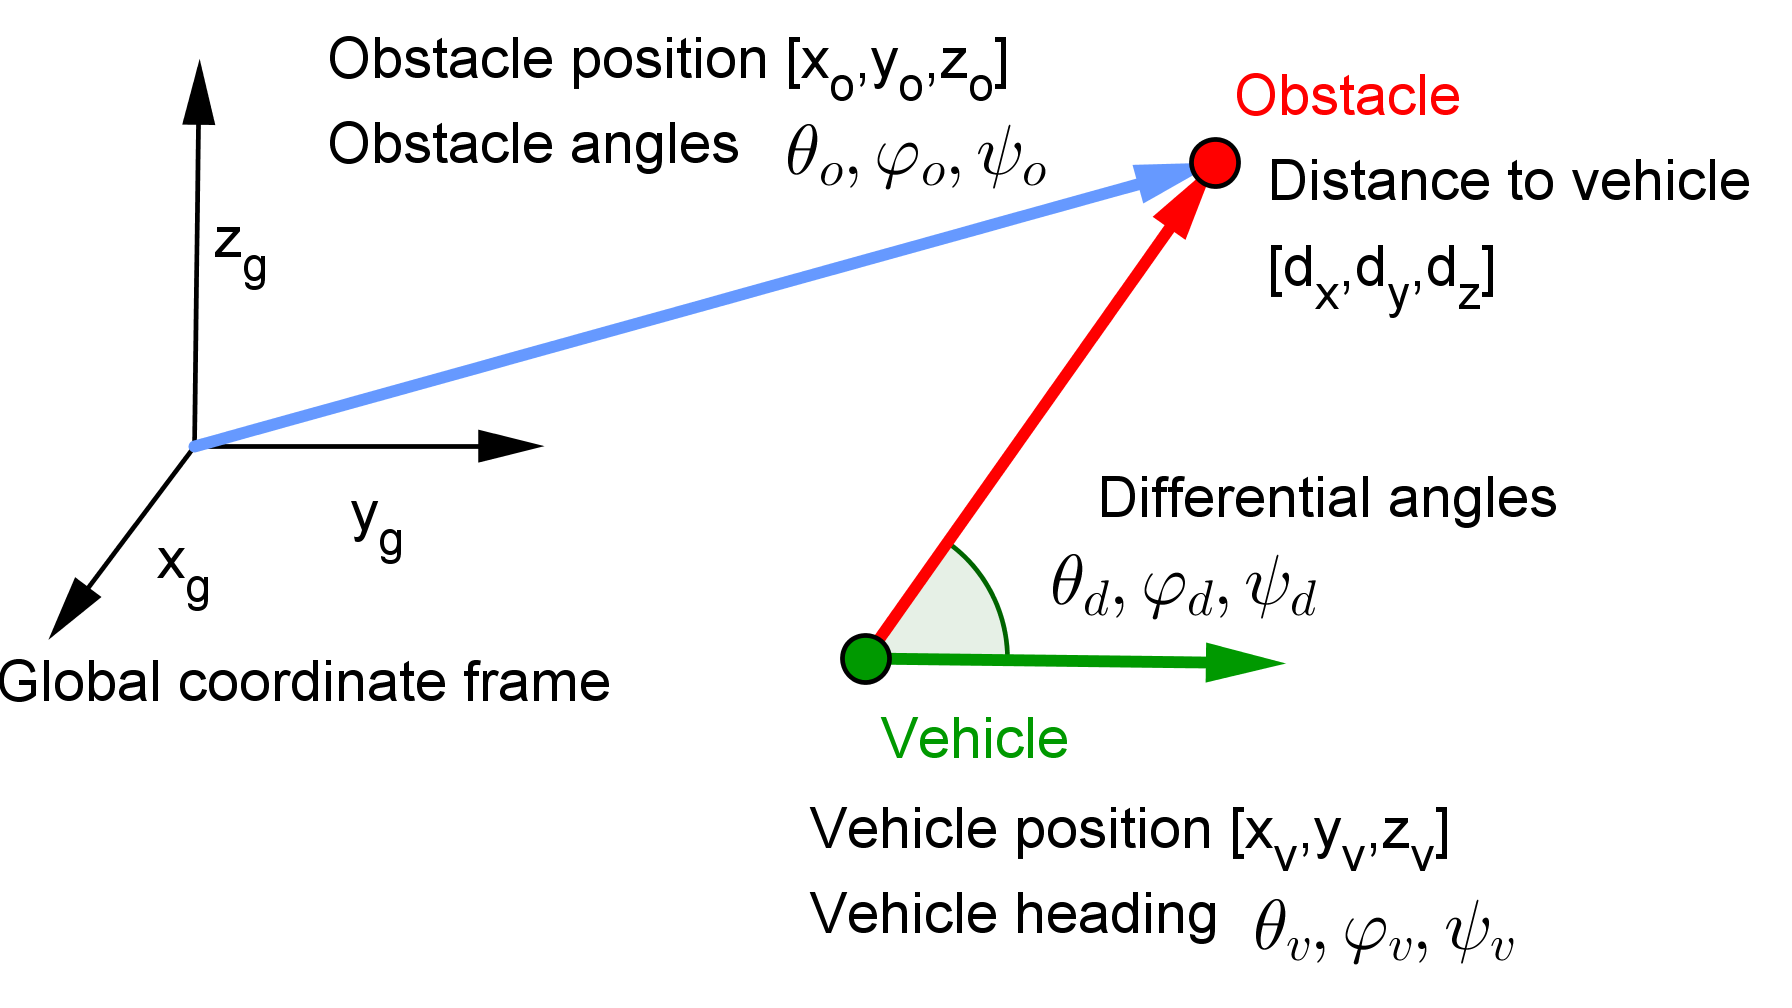
\includegraphics[width=0.55\linewidth]{\FIGDIR/63_Obstacle_Representation.png}
    \caption{Obstacle representation in $3D$ environment.}
    \label{fig:63ObstacleRepresentation}
\end{figure}

\noindent Where $[x_p,y_p,z_p]$ represents global coordinates of obstacle in known world $\mathscr{F}_{3D}$ , angles $\alpha,\beta,\gamma$ represents offset angles at YZ,XZ,XY, planes, differential angles $\delta_\alpha,\delta_\beta,\delta_\gamma$ represents angles definitions between orientation angles of plane $\alpha_v,\beta_v\gamma_v$, $do$ is distance to obstacle and $danger$ represents danger level\\
\newpage\noindent Distance $d_o$ is calculated as norm between obstacle position and vehicle position in global coordinate system, by following equation:
    \begin{equation}
        d_o = \norm{[x_o,y_o,z_o]^T-[x_v,y_v,z_v]^T}
    \end{equation}
Offset angles are calculated based on vehicle and obstacle position by following equations:
    \begin{equation}
        \alpha=\textnormal{atan2}(y_o-y_v,x_o-x_v)
    \end{equation}
    \begin{equation}
        \beta=\textnormal{atan2}(z_o-z_v,x_o-x_v)
    \end{equation}
    \begin{equation}
        \gamma=\textnormal{atan2}(z_o-z_v,y_o-y_v)
    \end{equation}
Differential angles are calculated based on vehicle orientation angles and obstacle offset angles, by following equations:
    \begin{equation}
        \delta_\alpha = \textnormal{atan2}(\sin(\alpha-\alpha_v),\cos(\alpha-\alpha_v))
    \end{equation}
    \begin{equation}
        \delta_\beta = \textnormal{atan2}(\sin(\beta-\beta_v),\cos(\beta-\beta_v))
    \end{equation}
    \begin{equation}
        \delta_\alpha = \textnormal{atan2}(\sin(\gamma-\gamma_v),\cos(\gamma-\gamma_v))
    \end{equation}
Danger level is calculated based on safety margin $s_m$, if $s_m$, if $d_o \ge s_m$ danger does not exist, otherwise if $\abs{\delta_\alpha} \le \pi, \abs{\delta_\beta} \le \pi, \abs{\delta_\gamma} \le \pi $ then direct hit danger is approaching otherwise turn hit danger is approaching. Danger level assessment function is defined in following equation:
    \begin{equation}
        danger = 
        \begin{cases}
            0:&d_o \ge s_m\quad\textnormal{ no danger}\\
            1:&d_o < s_m \textnormal{ and } \delta_\alpha,\delta_\beta,\delta_\gamma\in <-\pi/2,\pi/2> \\&\textnormal{direct hit danger}\\
            2:&d_o < s_m \quad\textnormal{ turn hit danger}\\
        \end{cases}
    \end{equation}

\end{definition}

\section{Control strategy}\label{sec:3DcontrolSimplisticStrategy}
\noindent Main purpose of control strategy is to define discrete set of moves which can be later used in approximation models. Therefore vehicle velocity is set to constant speed $v_v = 1\quad m/s$ because increasing and decreasing speed can make predicted trajectories malformed. It is needed to distinguish between \textit{control strategy} $\Omega(t)$ and \textit{control set} $U(t)$. \textit{Control set} $U(t)$ contains all available control inputs regardless vehicle state and surrounding. \textit{Control strategy} $\Omega(t)$ contains only control inputs $\omega(t)$ which keeps vehicle in safe invariant reachable set $\mathscr{R}$.
\begin{equation}\label{simple3dControlSet}
    u(t)\in U(T) =
    \begin{cases}
        \left [ v_c,0,0,0 \right ]^T & :s_0 \quad\textnormal{fly straight} \\
        \left [ v_c,0,\frac{\pi}{12},0 \right ]^T & :s_1 \quad\textnormal{fly downward} \\
        \left [ v_c,0,-\frac{\pi}{12},0 \right ]^T & :s_2 \quad\textnormal{fly upward} \\
        \left [ v_c,0,0,\frac{\pi}{12} \right ]^T & :s_3 \quad\textnormal{fly left} \\
        \left [ v_c,0,0,-\frac{\pi}{12} \right ]^T & :s_4 \quad\textnormal{fly right} 
    \end{cases}
\end{equation}
Control set $U(t)$ (\ref{simple3dControlSet}) contains five basic movement which affects yaw or pitch angular velocity. This allows us to develop movement set containing basic movement like fly straight, fly upward, fly downward, fly left and fly right. Movement set  is designed to cover maximum maneuverability. From viewpoint of reachable control set $U(t)$ have maximal maneuverability subset $\Gamma(t)$ which contains only maneuvers which are on border of reach set. Maximal maneuverability subset $\Gamma(t)$ is equal to control set $U(t)$ in this case. For example les sharp turn to right $u(t)=\left [ v_c,0,0,-\frac{\pi}{16} \right ]^T$ will be member of control set $U(t)$, but will not be member of maximal maneuverability set $\Gamma(t)$, because there exist sharper turn to right $u(t) = \left [ v_c,0,0,-\frac{\pi}{12} \right ]^T $. Maximal maneuverability set $\Gamma(t)$ is used in estimation of invariant safe reach set $\mathscr{R}$.

\section{Path finding in known environment}\label{ch:pathfindingInKnownEnviroment}
\noindent Abstractly, this is a constrained optimization problem where a feasible
trajectory $(x(t),u(t))$ that minimizes the cost function is found (\ref{eq:costFunction})
\begin{equation}\label{eq:costFunction}
    J =  L(x(t),u(t)) + V(x(T))
\end{equation}
The term $L(x,u)$ is referred to as the integral cost and V $(x(T))$ is the final (or terminal) cost. Definition of integral cost is simple it is summation of trajectory which have been flew, therefore integral cost is defined as trajectory flew in given time is defined by equation (\ref{eq:integral_cost})
\begin{equation}\label{eq:integral_cost}
    L(x(t),u(t)) = \int \norm{[\dot{x}_v(\tau),\dot{y}_v(\tau),\dot{z}_v(\tau)]^T}\quad d\tau
\end{equation}
Terminal cost function $V(x(T))$ must reflect penalization for not reaching goal waypoint. These functions are usually defined in form of penalty $\times$ coefficient, penalty can be seen as remaining shortest distance to goal (\ref{eq:distanceToGoalCalc}). Crashing to obstacle is penalized by $d_g$, when crash is inevitable $d_g=\infty$. Coefficient for final cost will be formulated as penalization function of vehicle orientation ($\alpha_v,\beta_v,\gamma_v$) and vector defined by start waypoint $\mathscr{W}_S$ and goal waypoint $\mathscr{W}_G$. The biggest difference between planar angles in absolute value is 180 degrees or $\pi$ radians. 
\begin{equation}\label{eq:penalizationCoeficient}
    \begin{aligned}
    p(\alpha_v,\beta_v,\gamma_v,\mathscr{W}_S,\mathscr{W}_G)= 1 +&\\
    +&\frac{\abs{\alpha_v -   \textnormal{atan2}(z_{\mathscr{W}_G}-z_{\mathscr{W}_S},y_{\mathscr{W}_G}-y_{\mathscr{W}_S})}}{\pi}\\
    +&\frac{\abs{\beta_v -   \textnormal{atan2}(z_{\mathscr{W}_G}-z_{\mathscr{W}_S},x_{\mathscr{W}_G}-x_{\mathscr{W}_S})}}{\pi}\\
    +&\frac{\abs{\alpha_v -   \textnormal{atan2}(y_{\mathscr{W}_G}-y_{\mathscr{W}_S},x_{\mathscr{W}_G}-x_{\mathscr{W}_S})}}{\pi}\\
    \end{aligned}
\end{equation}
Penalisation coefficient is given by (\ref{eq:penalizationCoeficient}) and with range $p(\dots)\in [1,4]$, therefore terminal cost of state in time $T$ can be given by equation (\ref{eq:terminalCost}).
\begin{equation}\label{eq:terminalCost}
    V(x(T)) = \int_{t_0}^\tau \dot{x}(s) +\dot{y}(s)+\dot{z}(s) ds + \norm{\begin{bmatrix}x(T)-x(\tau)\\y(T)-y(\tau)\\z(T)-z(\tau)\\ \end{bmatrix}}
\end{equation}
Terminal cost is represented as traveled path distance and direct distance to goal point $[x(T),y(T),z(T)]$ in time $\tau$.
\begin{figure}[H]
    \centering
    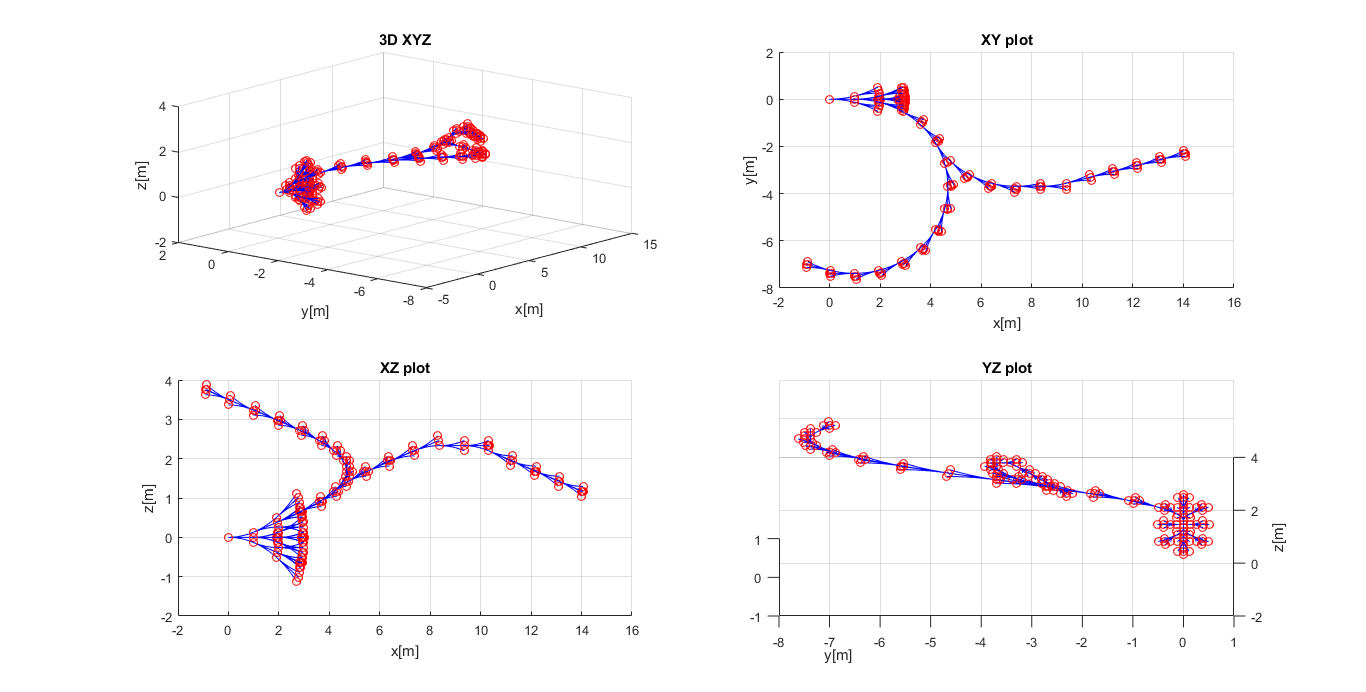
\includegraphics[width=0.75\linewidth]{\FIGDIR/58_Rapid_exploration_path_tree.png}
    \caption{Rapid path exploration tree example with weighted expand cost function $J^*$.}
    \label{fig:58rapidPathExploaation}
\end{figure}
\noindent Rapid path exploration method is method for finding feasible paths in known environment based on limited system dynamics $\dot{x}=f(x,u)$ where input belongs to control  set $u(t)\in U(T)$, example can be seen in figure \ref{fig:58rapidPathExploaation}.

Algorithm is based on tree search of possible movement nodes which represents vehicle state snapshots $x(t_i) i\in \N^+$. State snapshots are calculated based on predictive or linear model, to save computation time and calculation guarantees that real vehicle state $\hat{x}(t_i)$ will reach predicted state $x(t_i)$ with small perturbation $\epsilon$ therefore for each predicted state following inequality holds:
\begin{equation}\label{eq:marginalErrorofPrediction}
    \norm{\hat{x{t_i}}-x(t_i)}\le \epsilon^i,\quad i \in \N^+
\end{equation}
All possible paths $p$ in search tree are represented as sequence of nodes. Each node have defined parent, which is reference to previous node and leafs which are references to possible followers in path. For our purpose augmented data structure \textit{Node} will be presented with following properties:
\begin{enumerate}
    \item \textit{Movement} - movement which has been executed on this node.
    \item \textit{Goal distance} - distance to goal point in space calculated by (\ref{eq:distanceToGoalCalc}).
    \item \textit{Explored} - indication if node have been explored by stack execution true or false.
    \item \textit{Vehicle} - vehicle structure with state and obstacles situation.
    \item \textit{Parent} - parent node handle, if empty node is root of tree. 
    \item \textit{Leafs} - list of accessible non vehicle destructive leafs.
\end{enumerate}
\begin{equation}\label{eq:distanceToGoalCalc}
    d_{goal}(vehicle,\mathscr{W}_g) = 
    \begin{cases}
        \norm{\vec{x}_v-\vec{x}_{goal}}&:\nexists o \in \mathscr{O}; o.danger = 1 \vee 2\\
        \infty&:otherwise
    \end{cases}
\end{equation}
For purpose of rapid exploration limited move set needs to be introduced, therefore based on defined simplistic system model control set (\ref{simple3dControlSet}):
\begin{equation}\label{eq:rapidExplorationMovementSet}
    moveSet=
    \begin{cases}
        \left\{straight,left,right,up,down \right\} &: node.movement == straight\\
        \left\{straight,left, \right\} &: node.movement == left\\
        \left\{straight,right \right\} &: node.movement == right\\
        \left\{straight,up \right\} &: node.movement == up\\
        \left\{straight,down \right\} &: node.movement == down
    \end{cases}
\end{equation}
Goal of rapid exploration is to cover maximum amount of space without redundancy therefore allowed movement set \ref{eq:rapidExplorationMovementSet} is covering this situation. For example movement series $[right,left]$ returns to path given by movement series $[straight,straight]$, therefore possible movements after i finis $right$ movement are $right,straight$. This rule reduces search tree complexity from branching factor $n^5$ to branching factor $n^3$. Expand function represented by algorithm \ref{alg:03}.
\\
\begin{algorithm}[H]
\caption{Node expand(...) function.}
\label{alg:03}
\SetKwInOut{Input}{Input}\SetKwInOut{Output}{Output}
\Input{Node node}
\Output{Node[] leafs}
\If{isEmpty(node.leafs)}{
    \ForEach{$appliedMovement\in \left\{straight,left,right,up,down \right\}$}{
        newVehicle = vehicle.predictPosition(appliedMovement);\\
        Node child = new Node(vehicle);\\
        child.recalculateDistance();\\
        child.parrent = node;\\
        node.leafs.append(child);
    }
}
\end{algorithm}
Node selection is executed based on algorithm \ref{alg:04}. Not all leafs of expanded node can be exploration candidates, because some movements can lead to vehicle crash, which is represented by $node.goalDistance = \infty$. Other reason to decline leaf as exploration candidate is inappropriate movement, movement set which is based on parent node movement (\ref{eq:rapidExplorationMovementSet}), can allow only certain candidates to be explored. Other selection criteria based on system dynamics or constraints can be introduced into selection function later.

\begin{algorithm}[H]
    \caption{Node select(...) function.}
    \label{alg:04}
    \SetKwInOut{Input}{Input}\SetKwInOut{Output}{Output}
    \Input{Node node}
    \Output{Node[] candidates}
    candidates = [];\\
    \ForEach{leaf $\in$ node.leafs}{
    \If{leaf.movement $\in$ moveSet and leaf.goalDistance $\neq \infty$ and\\
        leaf.goalDistance $\le$ node.goalDistance and leaf.explored == false}{
            leaf.explored = true;\\
            candidates.append(leaf);
    }
}
\end{algorithm}
\newpage\noindent  Stack structure search is used for heuristic search of optimal path according to cost function (\ref{eq:costFunction}). Path given by heuristic algorithm \ref{alg:05}. is semi-optimal strongly depending on chosen time interval $t_i$ for prediction, count of predicted states $i$ and acceptable marginal error of prediction (\ref{eq:marginalErrorofPrediction}). Nevertheless its very fast and stable, and with limited search dynamics can cover large quantity of space, which makes it ideal candidate for obstacle avoidance in known environment. 

\begin{algorithm}[H]
    \caption{Search path function.}
    \label{alg:05}
    \SetKwInOut{Input}{Input}\SetKwInOut{Output}{Output}
    \Input{Node root, $\mathscr{WP}$ goal}
    \Output{Node path}
    stack = [root];
    \While{~isEmpty(stack)}{
        node = findBestCandidate(stack,goal); (\ref{eq:costFunction})\\
        node.expand($\dots$); (alg. \ref{alg:03}.)\\
        candidates = node.select($\dots$); (alg. \ref{alg:04}.)\\
        \ForEach{candidate $\in$ candidates}{
            \If{candidate.distance(goal) $\le$ marginDistance}{
                return candidate;
            }
        }
    }
\end{algorithm}

\section{Movement automaton predictor}\label{ch:movementAutomatonPredictor}
\noindent Vehicle system is given by model from section \ref{sec:3DsimplisticplaneModel}. Vehicle control is defined as movement automation $\mathscr{MA}$ with rapid exploration movement set defined in equation \ref{eq:rapidExplorationMovementSet}. Path exploration approach is given in section. 
\ref{ch:pathfindingInKnownEnviroment}. Movement predictor needs to be developed in order to obtain control signal $u(t)$ It is possible to predict movement buffer $B_{\mathscr{MA}}$, between vehicle initial position $x_0$ and waypoint, when known obstacle set $\mathscr{O}$ is given and movement state can be predicted for chain of movements. This approach have been defined in alg. \ref{alg:05}. as rapid exploration tree. Vehicle state $x(t_0)$ at start of mission execution is known. Vehicle state in discrete time $x(t)$ is given by equation \ref{eq:vehicleStateDiscreteKnown}. Where $x_v(t),y_v(t),z_v(t)$ is vehicle position in local coordinate frame and $\alpha_v(t),\beta_v(t),\gamma_v(t)$ is vehicle orientation angles.
\begin{equation}\label{eq:vehicleStateDiscreteKnown}
    x(t) = [x_v(t),y_v(t),z_v(t),\alpha_v(t),\beta_v(t),\gamma_v(t)]^T;
\end{equation}
Base movement table for movements $m_i(1)\in M$ have been measured on system model (\ref{sec:3DsimplisticplaneModel}). This table represents vehicle position and orientation differences after execution of movement. Vehicle initial state was set at center of local coordinate frame with narrow orientation $[x_0,y_0,z_0]=[0,0,0]$. Vehicle initial orientation was aligned with main frame axis X, therefore initial orientation angles are $[\alpha_0,\beta_0,\gamma_0] = [0,0,0]$. Vehicle velocity was set to constant value $v_v = 1 ms^{-1}$. Vehicle position after movement execution is given by parameters $x_b,y_b,z_b$ at time $t+1$. Vehicle orientation is given by parameters $\alpha_b,\beta_b,\gamma_b$. Givem parameters are also absolute shifting, because initial state is $[x_0,y_0,z_0,\alpha_b,\beta_b,\gamma_b]$ set to $\vec{0}$.
\begin{table}[H]
    \centering
    \begin{tabular}{|l||c|c|c|c|c|}
    \hline
        $v_x/m_i$           &    Straight $\circledcirc$ & Down $\Downarrow$  & Up $\Uparrow$    & Left $\Leftarrow$ & Right $\Rightarrow$\\\hline\hline
        $x_b [m]$           &    1.00	  & 0.98  & 0.98  & 0.98 & 0.98\\\hline
        $y_b [m]$           &    0	      & 0	  & 0	  & 0.13 & -0.13\\\hline
        $z_b [m]$           &    0	      & -0.13 & 0.13  &	0	 & 0\\\hline
        $\alpha_b [rad]$	&    0	      & 0	  & 0	  & 0    & 0\\\hline
        $\beta_b [rad]$     &    0	      & 0.2   & -0.26 & 0	 & 0\\\hline
        $\gamma_b [rad]$    &    0	      & 0	  & 0	  & 0.26 & -0.26\\\hline
    \end{tabular}
    \caption{Base values for movement application, vehicle position difference $x_v,y_v,z_v$ and orientation differences $\alpha_v,\beta_v,\gamma_v$.}
    \label{tab:movementPredictor}
\end{table}
\noindent With defined base movement table (tab. \ref{tab:movementPredictor}). with defined shifting for movement at time $t_0+1$, \textit{rotation} (\ref{eq:rotationSimplisticPredictor}) and \textit{shifting} (\ref{eq:shiftingSimplisticPredictor}) equations must be defined in order to obtain predicted position $\hat{x}(t+1)$. Position after movement execution $[\hat{x}(t+1),\hat{y}(t+1),\hat{z}(t+1)]$ is depending on vehicle orientation before movement execution $[\alpha_v(t),\beta_v(t),\gamma_v(t)]$. Rotation function rotates vehicle position $[x_b(t_0),y_b(t_0),z_b(t_0)]$ according to vehicle orientation angles $[\alpha_v(t),\beta_v(t),\gamma_v(t)]$. For rotation standard rotation matrix $R_{XYZ}(\alpha,\beta\gamma)$ (\ref{eq:xyzspaceRotationMatrix}) is used. Final position offset vector $[\tilde{x}_b(t+1),\tilde{y}_b(t+1),\tilde{z}_b(t+1)]$ at predicted time $t+1$ is given by equation \ref{eq:rotationSimplisticPredictor}.
\begin{equation}\label{eq:rotationSimplisticPredictor}
    \begin{bmatrix}
        \tilde{x}_b\\ 
        \tilde{y}_b\\
        \tilde{z}_b\\
    \end{bmatrix}
    = R_{XYZ}(\alpha_v(t),\beta_v(t),\gamma_v(t))
    \begin{bmatrix}
        x_b\\ 
        y_b\\
        z_b\\
    \end{bmatrix}
\end{equation}
Predicted state vector $\hat{x}(t+1)$ a at time $t+1$ is obtained by combining position offset vector $[\tilde{x}_b(t+1),\tilde{y}_b(t+1),\tilde{z}_b(t+1)]$, orientation offset vector $\alpha_b(t+1),\beta_b(t+1),\gamma_b(t+1)$. as given in equation \ref{eq:shiftingSimplisticPredictor}.
\begin{equation}\label{eq:shiftingSimplisticPredictor}
    \begin{aligned}
    \hat{x}(t+1) & = [\hat{x}_v(t+1),\hat{y}_v(t+1),\hat{z}_v(t+1),\hat{\alpha}_v(t+1),\hat{\beta}_v(t),\hat{\gamma}_v(t)]^T\\
    \hat{x}_v(t+1) & = x_v(t)+\tilde{x}_b\\
    \hat{y}_v(t+1) & = y_v(t)+\tilde{y}_b\\
    \hat{z}_v(t+1) & = z_v(t)+\tilde{z}_b\\
    \hat{\alpha}_v(t+1) & = \alpha_v(t) + \alpha_b\\
    \hat{\beta}_v(t+1) & = \beta_v(t) + \beta_b\\
    \hat{\gamma}_v(t+1) & = \gamma_v(t) + \gamma_b
    \end{aligned}
\end{equation}
Movement automaton $\mathscr{MA}$ has chaining property, therefore movement prediction chaining is also possible via recursive procedure for discrete execution time $t_i$. There exist predicted movement buffer $\hat{B}$ with ordered movement sequence $m_1(1),\dots,m_i(1)$, vehicle state after applying movement $m_{i+1}$ at time $t_i$ can be obtained via equation \ref{eq:discretePredictionChaining}.
\begin{equation}\label{eq:discretePredictionChaining}
    \hat{x}(t_i+1) = f(\hat{x}(t_i),m_{i+1}(1))
\end{equation}
Prediction function $f(\hat{x}(t_i),m_{i+1}(1))$ is in this case function defined by equation \ref{eq:shiftingSimplisticPredictor}, where parameters $[x_b,y_b,z_b,\alpha_b,\beta_b\gamma_b]$ are selected based on movement $m_{i+1}(1)$ type from lookup table  \ref{tab:movementPredictor}.


